% Copyright (C) The IMR developers. SPDX-License-Identifier: GPL-3.0-or-later
\documentclass[tikz,border=8pt]{standalone}
\usepackage[T1]{fontenc}
\usepackage{lmodern}
\usetikzlibrary{arrows.meta}
\definecolor{ink}{HTML}{122D4A}
\definecolor{wave}{HTML}{2776C9}
\definecolor{heat}{HTML}{DF8D32}
\definecolor{rheo}{HTML}{168B88}
\begin{document}
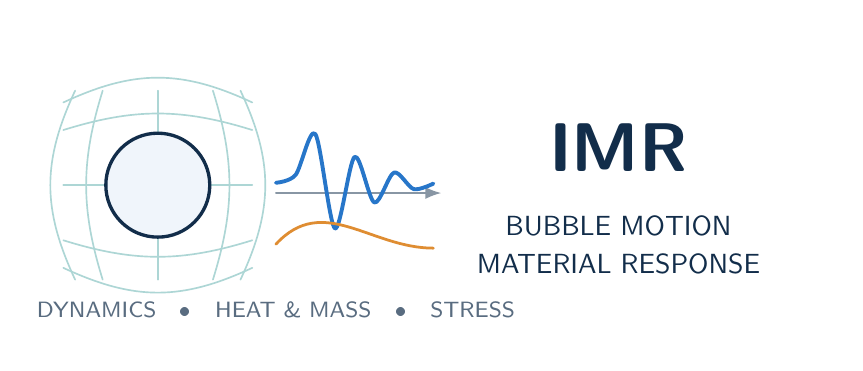
\begin{tikzpicture}[>=Latex,font=\sffamily,line cap=round,line join=round]
  \fill[white] (-1.6,-2) rectangle (8.6,2);
  \foreach \x in {-1.05,-.7,0,.7,1.05}
    \draw[rheo!35,line width=.6pt] (\x,-1.2) .. controls (\x*1.4,-.3) and (\x*1.4,.3) .. (\x,1.2);
  \foreach \y in {-1.05,-.7,0,.7,1.05}
    \draw[rheo!35,line width=.6pt] (-1.2,\y) .. controls (-.3,\y*1.4) and (.3,\y*1.4) .. (1.2,\y);
  \fill[white] (0,0) circle (.66);
  \fill[wave!7] (0,0) circle (.66);
  \draw[ink,line width=1.2pt] (0,0) circle (.66);
  \draw[->,ink!50,line width=.6pt] (1.5,-.1) -- (3.6,-.1);
  \draw[wave,line width=1.4pt] plot[smooth] coordinates {(1.5,.03) (1.75,.13) (2,.65) (2.25,-.55) (2.5,.36) (2.75,-.22) (3,.16) (3.25,-.05) (3.5,.02)};
  \draw[heat,line width=1pt] (1.5,-.75) .. controls (2.1,-.1) and (2.7,-.8) .. (3.5,-.8);
  \node[text=ink,font=\sffamily\bfseries\fontsize{45}{49}\selectfont] at (5.85,.48) {IMR};
  \node[text=ink,font=\sffamily\fontsize{10}{14}\selectfont,align=center] at (5.85,-.76)
    {BUBBLE MOTION\\MATERIAL RESPONSE};
  \node[text=ink!70,font=\sffamily\fontsize{8}{10}\selectfont] at (1.5,-1.58)
    {DYNAMICS\quad\textbullet\quad HEAT \& MASS\quad\textbullet\quad STRESS};
\end{tikzpicture}
\end{document}
